\chapter{Towards reactive mobile application development}\label{towards-reactive-mobile-application-development}

The first chapter introduced the literature and the main concepts of the
RP paradigm, and the second one depicted some of the main popular and
used libraries and framework for RP. This chapter will propose a
concrete applications of the paradigm to some practical use cases that
recur pretty frequently when developing mobile application nowadays.

Thus, this chapter will focus its attention on mobile application
development, in both the Android and iOS platforms.

The main idea that brings RP to mobile application development is in the
abstraction that considers an app as a function, or as a flow of user
inputs that are continuously evaluated, filtered, combined, and so on,
producing a some sort of outputs and effects.


\section{Abstracting the retrieval, manipulation and presentation of
data}\label{abstracting-the-retrieval-manipulation-and-presentation-of-data}

The first use case proposed is about a quite common set of actions, such
as the \textbf{retrieval, manipulation and presentation of some sort of
data}.

Every simple or complex application has at least a part in the app
lifecycle in which it queries some provider (a cache, a local database,
a Rest API) to fetch some resource, so this initial use case can be
considered as a foundational building block for every application.

The abstraction of event streams can be used to model this use case in a
pretty straight-forward way.

In the case of a web request, the stream will either emit one value -
containing the body of the response - and succeed, or fail with an error.

In the case of more complex request-response configuration (e.g.~a
request that opens a websocket, that then emits and push new data over
a long time) the stream will emit more values, as long as the flow of
items continues, or terminate if a failure occurs.

Abstracting the reception of items is only the first part of the
scenario introduced. Once the application got some kind of data, a
certain number of processing stages can be run over these data. Thus,
the notion of event streams and operators fits really nicely also on
this part.

To demonstrate a possible solution of this scenario using an approach
based on RP, lets introduce a sample use case:

\begin{quote}
The application has to query a webservice, that returns a list of words
for a given month. Each word refers to a specific day, month and year.
The application should show all the words in the given month, sorted by
date, with the first one highlighted with a different color.
\end{quote}

\subsection{On Android}\label{on-android}

After introducing the use case, the first thing to do is to write down
the types involved in the computation and to provide a class that
handles the network requests, returning an observable with the response.
This class will be part of the network layer of the application, and
will expose methods like the following:

\begin{verbatim}
public Observable<List<Word>> getWords(int month, int year);
\end{verbatim}

As a reference, the \texttt{Word} type is the following:

\begin{verbatim}
public class Word {
    public long id;
    public String word;
    public int day;
    public int month;
    public int year;
}
\end{verbatim}

The semantics for this observable is pretty simple:

\begin{itemize}
\itemsep1pt\parskip0pt\parsep0pt
\item
  it \emph{yields} a single results (the response body) or an error (a
  network error, or a server error, etc..)
\item
  it \emph{starts} the computation each times a consumer
  \emph{subscribes} itself to the observable
\end{itemize}

NB: for this kind of request, the behavior would also have been
implemented with a future.

Once the network layer is in place, all the transformation needed can be
expressed in term of operators.

\begin{verbatim}
myServiceProvider.getWords(month, year)

    // network operations in io scheduler
    .subscribeOn(Schedulers.io())

    // Observable<List<Word>> -> Observable<Word>
    .flatMap(wordList -> Observable.from(wordList))

    // sort elements
    .toSortedList((l, r) -> { ...sort predicate... })

    // Observable<List<Word>> -> Observable<Word>
    .flatMap(list -> Observable.from(list))

    // build an Observable<Pair<Integer, Word>> 
    // (the integer value is the index)
    .map(word -> new Pair<>(0, word))
    .scan((sum, item) -> new Pair<>(sum.first + 1, item.second))

    // build list adapter, highlighting the first element
    // Observable<Pair<Integer, Word>> -> Observable<WordListItem>
    .map(indexItemPair -> { 
        WordListAdapter.WordListItem item 
        	= new WordListAdapter.WordListItem(indexItemPair.second);
        item.setHighlighted(...); // highlight current day item
        return item;
    })
    .toList() // converting to list, since the adapter need a list

    //  UI update on main thread
    .observeOn(AndroidSchedulers.mainThread())

    // subscribing to items, errors, ...
    .subscribe(
        wordItemList -> {
            setListAdapter(
            	new WordListAdapter(wordListActivity, wordItemList));
        },
        throwable -> {
        ...
        }
    );
\end{verbatim}

The code shows some transformations and some usage of the most common
operators of RxJava.

In the code snippet, \texttt{flatMap} is used to transform an
\texttt{Observable\textless{}List\textless{}Word\textgreater{}\textgreater{}}
to an \texttt{Observable\textless{}Word\textgreater{}}. This is a pretty
common transformation when dealing with list of elements, and since
operators like \texttt{map}, \texttt{filter}, etc.. need to operate on
single elements, this operation is essential to build the chain.

Another pattern is the usage of \texttt{map} in conjunction with
\texttt{scan}, to accumulate the result of a computation. The code
presented does the trivial job of associating to each element its index
in the observable, but it's a use case useful enough to deserve a
citation.

The presentation of the items is provided by the
\texttt{WordListAdapter} and \texttt{WordListItem} classes.

One last things to note is the usage of \texttt{subscribeOn} and
\texttt{observeOn}, to keep the main thread responsive.

\subsection{On iOS}\label{on-ios}

On iOS, the problem can be solved using the same conceptual
abstractions.

Starting with a network provider that expose the call to the APIs with
the following method signature:

\begin{verbatim}
func getWords(month: Int, year: Int) -> SignalProducer<[Word], NSError>
\end{verbatim}

As a reference, the type \texttt{Word} is defined as follows:

\begin{verbatim}
public struct Word {

    public let id: Int
    public let word: String
    public let day: Int
    public let month: Int
    public let year: Int

    init(id: Int, word: String, day: Int, month: Int, year: Int){
        self.id = id
        self.word = word
        self.day = day
        self.month = month
        self.year = year
    }
}
\end{verbatim}

Also on iOS, the semantics for this signal producer is pretty simple and
similar to the android counterpart:

\begin{itemize}
\itemsep1pt\parskip0pt\parsep0pt
\item
  it \emph{yields} a single results (the response body) or an error (a
  network error, or a server error, etc..)
\item
  it \emph{starts} the computation each times a consumer
  \emph{subscribes} itself on the signal producer
\end{itemize}

\begin{verbatim}
getWords(month, year)
    // sort
    |> map { words in words.sorted(...) }

    // SignalProducer<[Word]> -> SignalProducer<Word>
    |> flatMap(FlattenStrategy.Merge, { 
    	words in SignalProducer(values: words) })

    // build an SignalProducer<(Int, Word)>
    // (the integer value is the index)
    |> map { word in (0, word) }
    |> scan( (0, nil), { (last, current) in (last.0 + 1, current.1) })

    // observe on UI thread
    |> observeOn(UIScheduler())

    // start and subscribe to elements, errors, ...
    |> start(next: { elem in self.updateView(elem)})
\end{verbatim}

Almost every step of the chain is the same as its android counterpart.
The main difference is that RAC doesn't offer a method to sort the
elements of a SignalProducer, so, in this case, the elements are
filtered at the beginning of the chain using a method of the
\texttt{Array} type.


\section{Choosing an architectural
pattern}\label{choosing-an-architectural-pattern}

This section will explore a fundamental aspect of mobile application
development: the architectural pattern.

When developing a mobile applications, usually the target platform
implicitly or explicitly suggests an architecture.

\subsection{State of the art in iOS}\label{state-of-the-art-in-ios}

In the iOS world, Apple encourages the usage of the
Model-View-Controller (MVC) architectural pattern. Quoting the ``Start
Developing iOS Apps Today'' Apple's documentation:

\begin{quote}
\textbf{MVC} assigns the objects in an app to one of three roles:
\textbf{model}, \textbf{view}, or \textbf{controller}. In this pattern,
models \emph{keep track} of your app's data, views \emph{display} your
user interface and \emph{make up the content} of an app, and controllers
\emph{manage} your views. By responding to user actions and populating
views with content from the data model, controllers serve as a
\emph{gateway} for communication between the model and views.
\end{quote}

\begin{figure}[htbp]
\centering
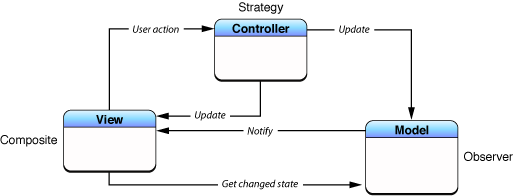
\includegraphics[scale=0.75]{imgs/ios_traditional_mvc.png}
\caption{Traditional MVC in iOS}
\end{figure}

In its original abstraction, in MVC:

\begin{itemize}
\itemsep1pt\parskip0pt\parsep0pt
\item
  the user manipulates a view and, as a result, an event is generated
\item
  a controller receives the event and manage apply an
  application-specific strategy
\item
  this strategy can consist in requesting a model object to update its
  state or in requesting a view object to change its appearance.
\item
  the model object notifies all objects who have registered as observers
  when its state changes; if the observer is a view object, it may
  update its appearance accordingly.
\end{itemize}

\begin{figure}[htbp]
\centering
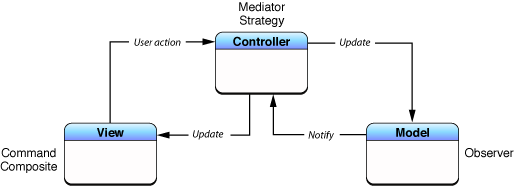
\includegraphics[scale=0.75]{imgs/cocoa_mvc.png}
\caption{Cocoa version of MVC}
\end{figure}

However, in an attempt to enhance code reusability, Apple suggests
developers to adopt a modified version of MVC, in which there's a strong
isolation from models and views, and in which controllers act an
intermediary between one or more of an application's view objects and
one or more of its model objects.

Even if views and view controllers are technically distinct components
and Apple suggests to keep these decoupled, they are almost always
paired. There are a lot reason that cause this trend of strictly
coupling a view and its controller:

\begin{itemize}
\itemsep1pt\parskip0pt\parsep0pt
\item
  the framework provides a big set of components in which a controller
  already has and manages a view (\texttt{UIViewController},
  \texttt{UITableViewController}, \texttt{UICollectionViewController},
  \texttt{UISplitViewController}, \texttt{TabBarController}, \ldots{})
\item
  the UIViewController class usually contains a lot of UI-related code
\item
  storyboards, that enable developers or designers to define GUIs,
  reason in term of view controllers and ``segue'' between view
  controllers
\end{itemize}

With this said, it is reasonable to modify the previous model with an
update in which the view and the view controller are paired together.

\begin{figure}[htbp]
\centering
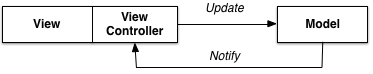
\includegraphics[scale=0.75]{imgs/real_mvc.png}
\caption{A revised iOS application architecture, in which the view and
the controller are coupled}
\end{figure}

The iOS community, during the years, has adopted (also unconsciously)
this architectural pattern to design applications. This has often lead
to what is called the ``Massive View Controller'' anti-pattern. The term
``Massive'' is used to denote the use and abuse of the view controller
entity to host most of the application logic, grouping functionalities
that don't strictly relate to the controller entity.

\subsection{State of the art in
Android}\label{state-of-the-art-in-android}

Android's documentation is less explicit about the architectural pattern
that developers should use.

At first sight, the overall architecture looks similar at iOS's
architecture, with the notion of \texttt{Activity} that is similar to
\texttt{UIViewController} and the notion of \texttt{View} that is
similar to \texttt{UIView}.

But, more in depth, things are far more complicated. Thus, the main flaw
comes from the assumption that there should be only one running
\texttt{Activity} at a time, and that this \texttt{Activity} should be
tied down to a single main view. To overcome this limitation, Android
introduced the \texttt{Fragment} class. This new abstraction allows an
activity to show and manage a certain number of fragments, but still has
some limitations like, for example, the possibility of manage stack of
fragments.

From this point of view, the iOS platform offers a clearer abstractions,
with the notion of viewcontrollers, views and viewcontroller containers,
that allow the developer to express multi-level view hierarchy in a
cleaner way.

Many developers suggest that what Android is offering is a broken
abstraction.

Knowing the limitations of the abstractions that the platform offers,
the most popular architectural pattern for Android is a variant of MVC
(similar to Apple's variant), in which the \texttt{Activity} (and
related fragments) is both a the view and the controller. Google
encourages developers to split each view in a fragment, and then each
fragment should interact with its parent activity, also to coordinate
his actions and commands with other fragments.

\subsection{Toward a common architecture:
MVVM}\label{toward-a-common-architecture-mvvm}

On both the platforms, the MVC architectural pattern and its variations
doesn't seem to be a perfect fit.

In this section and in the following ones a new architectural pattern
will be proposed to better model mobile applications: the
\textbf{Model-View-ViewModel} pattern.

The reason of the introduction of MVVM in this thesis is that this
pattern is an application pattern that isolates the user interface from
the underlying business logic, and, as introduced in the previous
section, one of the biggest issue of the usage of the MVC pattern is the
fact that in both Android and iOS there's not a clear distinction
between the view and the controller entities.

The MVVM pattern consists of the following parts:

\begin{itemize}
\itemsep1pt\parskip0pt\parsep0pt
\item
  the \textbf{Model}, which provides a view-independent representation
  of business entities;
\item
  the \textbf{View}, which is the user interface, displaying information
  to the user and firing events in response to user interactions;
\item
  the \textbf{ViewModel}, which is the bridge between the view and the
  model. Each View has at least a corresponding ViewModel. The ViewModel
  retrieves data from the Model and manipulates it into the format
  required by the View, wrapping the presentation logic. It notifies the
  View if the underlying data in the model is changed, and it updates
  the data in the Model in response to UI events from the View.
\end{itemize}

\begin{figure}[htbp]
\centering
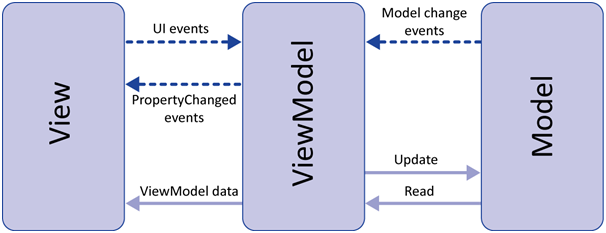
\includegraphics[scale=0.75]{imgs/mvvm.png}
\caption{The MVVM architectural pattern}
\end{figure}

Looking at the diagram, it's clear that the view-model:

\begin{itemize}
\itemsep1pt\parskip0pt\parsep0pt
\item
  sits between the model and the view, \textbf{wrapping all the
  presentation logic}
\item
  receives the events and commands from the view
\item
  \textbf{updates the view} once the model has been updated
\end{itemize}

The main reason to use MVVM is the it \textbf{reduces the complexity} of
one's viewcontrollers or activities and makes one's presentation logic
easier to test.

RP frameworks are a good fit in MVVM, since they allow to \textbf{bind
the views with their associated view-models}, allowing the proper
\textbf{synchronization} to reflect the changes in both directions.

\section{A case study}\label{a-case-study}

To illustrate the application of the MVVM pattern in conjunction with RP
frameworks, let's introduce a simple-but-effective use case.

The use case is an app for iOS and Android, that will:

\begin{itemize}
\itemsep1pt\parskip0pt\parsep0pt
\item
  fetch a web service to request a list of words;
\item
  each words has a set of attributes, such as: an id, a title, a day, a
  month and a year which is related to, and an url to an image;
\item
  after querying the web service, the result should be showed in a list.
  Each list item should display all the attributes, with also the image;
\item
  a detail view should be opened when the user taps on an item.
\end{itemize}

The requirements are pretty trivial for an experienced developer that
use to work following the ``standard'' way to develop mobile
applications, but in this thesis author's opinion is a pretty
significative example, since it allows to demonstrate a lot of concepts:

\begin{itemize}
\itemsep1pt\parskip0pt\parsep0pt
\item
  abstracting the retrieval, manipulation and presentation of data (also
  see the previous dedicated section);
\item
  presenting an uniform abstraction, applicable on both the platforms;
\item
  proper separation of concerns, applying MVVM.
\end{itemize}


\subsection{A common architecture}\label{a-common-architecture}

Starting from the requirements and with \textbf{MVVM} in mind, what
follows is the proposed overall system architecture.

\begin{figure}[htbp]
\centering
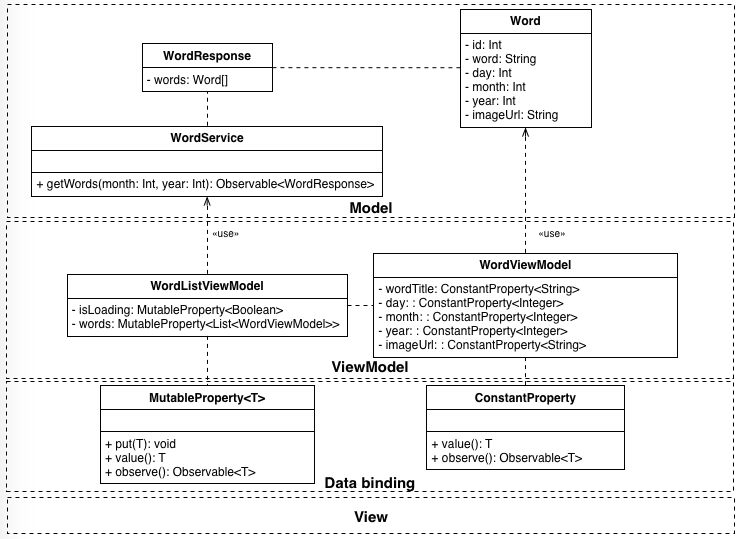
\includegraphics[scale=0.5]{imgs/common_arch.png}
\caption{The overall architecture}
\end{figure}

NB: the diagram is incomplete, and shows only the relevant building
block of the system. The convention used here to express the abstraction
of stream of items is the RxJava's \texttt{Observable} type.

What immediately emerges looking at the diagram is how the MVVM pattern
is applied to model the requirements.

The \textbf{Model} provides a view-independent representation of the
business entities. In this case, it's pretty trivial to express the
model of the Word class.

The \textbf{View} doesn't show something relevant at this stage, since
it heavily depends on platform-specific abstractions, and for this
reason it will be better depicted in the next two sections.

The \textbf{ViewModel} is the bridge between the view and the model,
wrapping all the presentation logic. In particular, there are two
concrete type of viewmodels:

\begin{itemize}
\itemsep1pt\parskip0pt\parsep0pt
\item
  \texttt{WordListViewModel}, that represent the viewmodel for the list
  view, as a whole;
\item
  \texttt{WordViewModel}, that represent the viewmodel for a single item
  of the list.
\end{itemize}

\texttt{WordListViewModel} use a \texttt{WordService}, that is a class
that wraps all the network and parsing operations, returning a
\texttt{WordResponse}, that contains an array of \texttt{Word}.
\texttt{WordListViewModel} has two \texttt{MutableProperty}:

\begin{itemize}
\itemsep1pt\parskip0pt\parsep0pt
\item
  \texttt{isLoading}, that indicates if there's a fetch request running
\item
  \texttt{words}, that contains the updated list of words
\end{itemize}

\texttt{WordViewModel} is a pretty simple entity, only containing some
\texttt{ConstantProperty}, referring to the word attributes. The number
of instances of \texttt{WordViewModel} will be equal to the number of
\texttt{Word} returned by the \texttt{WordService}.

\texttt{MutableProperty} and \texttt{ConstantProperty} are two
abstractions that help in binding the viewmodel to the view, allowing to
set up the automatic update of the view layer when the model gets
updated.

Note that this architecture is platform-agnostic and there are no
reference to a specific platform or native abstractions, except for the
\texttt{Observable} type (which can be easily traduced in
\texttt{SignalProducer}, in this specific context).

\subsubsection{Is this RP?}\label{is-this-rp}

Looking at the whole architecture, a question may arise. Is this RP?

The answer to this question is not trivial, at first glance. In the
introduced architecture RP abstraction are used as building block to
compose the overall architecture.

For example, the \texttt{WordService} class returns an
\texttt{Observable}. This immediately suggests a whole set of
considerations about the underlying computation.

Another example are the \texttt{MutableProperty} and
\texttt{ConstantProperty} classes, that under the hood are implemented
as \texttt{Subject} (or \texttt{Signal/SignalProducer}).

In conclusion, RP abstractions can be used as means to properly build
the overall architecture.


\subsection{Implementation on Android}\label{implementation-on-android}

The previous section proposed an overall architecture for the use case.
This sections will depict a possible implementation for the Android
platform.

\subsubsection{Model}\label{model}

Starting from the \textbf{model}, things are pretty straightforward.

The \texttt{Word} type only contains some read-only properties and a
constructor.

\begin{verbatim}
public class Word {

    public final long id;
    public final String word;
    public final int day;
    public final int month;
    public final int year;
    public final String imageUrl;

    public Word(int id, String word, int day,
        int month, int year, String imageUrl) {

        this.id = id;
        this.word = word;
        this.day = day;
        this.month = month;
        this.year = year;
        this.imageUrl = imageUrl;
    }
}
\end{verbatim}

The \texttt{WordResponse} class only wraps an array of \texttt{Word},
and also the logic for failed requests (that is omitted for the sake of
concisness).

\begin{verbatim}
public class WordResponse {
    final public Word[] words;
    WordResponse(Word[] words) {
        this.words = words;
    }
}
\end{verbatim}

Finally, the \texttt{WordService} class only expose a public method that
returns an \texttt{Observable\textless{}WordResponse\textgreater{}}.
Also in this case, the real implementation of this method is not
important for the purpose of this thesis, and it's omitted. The real
important thing of this class is the return type of the method
signature.

\begin{verbatim}
public class WordService {
    public WordService() { ... }
    public Observable<WordResponse>
        getWords(int month, int year) {
        ...
    }
}
\end{verbatim}

\subsubsection{Data binding}\label{data-binding}

To better understand the following steps, it's necessary to introduce
the abstraction of \texttt{MutableProperty} and
\texttt{ConstantProperty}. On the iOS counterpart, ReactiveCocoa already
offers the corresponding abstraction. RxJava and RxAndroid don't
directly offer the conceptual equivalent, but it's pretty easy to build
the same abstraction starting from a \texttt{BehaviorSubject}.

\begin{verbatim}
public interface Val<T> {
    T value();

    boolean hasValue();

    Observable<T> observe();
}
\end{verbatim}

The \texttt{Val} interface introduces the notion of a \textbf{value} of
type \texttt{T}.

\begin{verbatim}
public interface Var<T> extends Val<T> {
    void put(T value);
}
\end{verbatim}

The \texttt{Var} interface introduces a \textbf{variable} of a type
\texttt{T}.

\begin{verbatim}
public class MutableProperty<T> implements Var<T> {
    private final BehaviorSubject<T> subject;
    private Val<T> val;

    protected MutableProperty() {
        subject = BehaviorSubject.create();
    }

    protected MutableProperty(T defaultValue) {
        subject = BehaviorSubject.create(defaultValue);
    }

    public static <T> MutableProperty<T> create() {
        return new MutableProperty<>();
    }

    public static <T> MutableProperty<T> create(T defaultValue) {
        return new MutableProperty<>(defaultValue);
    }

    @Override public void put(T value) {
        subject.onNext(value);
    }

    @Override public synchronized Val<T> asVal() {
        if (val == null) {
            val = ConstantProperty.of(this);
        }

        return val;
    }

    @Override public T value() {
        return subject.getValue();
    }

    @Override public boolean hasValue() {
        return subject.hasValue();
    }

    @Override public Observable<T> observe() {
        return subject.asObservable();
    }
}
\end{verbatim}

The \texttt{MutableProperty} implements the \texttt{Var} interface, and
represents the abstraction of a property that is \textbf{updated over
the time}. This kind of property has a notion of current value (that can
also be absent) and can be observed, returning an \texttt{Observable}.

\begin{verbatim}
public class ConstantProperty<T> implements Val<T> {
    private final Var<T> var;

    protected ConstantProperty(Var<T> var) {
        this.var = var;
    }

    public static <T> ConstantProperty<T> of(Var<T> var) {
        return new ConstantProperty<>(var);
    }

    public static <T> ConstantProperty<T> create(T val) {
        return ConstantProperty.of(new MutableProperty(val));
    }

    @Override public T value() {
        return var.value();
    }

    @Override public boolean hasValue() {
        return var.hasValue();
    }

    @Override public Observable<T> observe() {
        return var.observe();
    }
}
\end{verbatim}

The \texttt{ConstantProperty} implement a property that can have a
single-assignment (constant) value.

\subsubsection{ViewModel}\label{viewmodel}

Moving to the viewmodel layer, things starts to become interesting.

\begin{verbatim}
public class WordListViewModel {

    private static final String TAG 
    	= WordListViewModel.class.getSimpleName();

    public final MutableProperty<Boolean> isLoading =
        MutableProperty.create(false);
    public final MutableProperty<List<WordViewModel>> words =
        MutableProperty.create(new LinkedList<>());

    public WordListViewModel(WordService wordService) {

        wordService.getWords(1, 2015)
                .doOnSubscribe(() -> this.isLoading.put(true))
                .observeOn(AndroidSchedulers.mainThread())
                .flatMap(wordResponse ->
                    Observable.from(wordResponse.words))
                .map(word -> new WordViewModel(word))
                .toList()
                .subscribe(wordViewModelList -> {
                            this.isLoading.put(false);
                            this.words.put(wordViewModelList);
                        },
                        throwable -> {
                            this.isLoading.put(false);
                            Log.e(TAG, throwable.getMessage());
                        });
    }
}
\end{verbatim}

As previously introduced in the architecture diagram, the
\texttt{WordListViewModel} class has two public
\texttt{MutableProperties} and exposes a constructor that receives a
\texttt{WordService}.

When an instance of \texttt{WordListViewModel} is created, the viewmodel
provides to build the chain of computations needed to perform its job.
In this case, it starts a fetch request using the \texttt{WordService}
instance, and then setting all the proper side-effects.

If everything completes fine, the two mutable properties are updated as
follows:

\begin{itemize}
\itemsep1pt\parskip0pt\parsep0pt
\item
  in \texttt{isLoading} is put \texttt{false}, so any view that observe
  that property will be notified of the termination of the request
\item
  in \texttt{words} is put a List
\end{itemize}

\begin{verbatim}
public class WordViewModel {

    final public ConstantProperty<String> wordTitle;
    final public ConstantProperty<Integer> day;
    final public ConstantProperty<Integer> month;
    final public ConstantProperty<Integer> year;
    final public ConstantProperty<String> imageUrl;

    public WordViewModel(Word word) {
        this.wordTitle = ConstantProperty.create(word.word);
        this.day = ConstantProperty.create(word.day);
        this.month = ConstantProperty.create(word.month);
        this.year = ConstantProperty.create(word.year);
        this.imageUrl = ConstantProperty.create(word.imageUrl);
    }
}
\end{verbatim}

The \texttt{WordViewModel} class is even simpler, since it only contains
a set of \texttt{ConstantProperty}, abstracting the set of attributes of
the \texttt{Word} class.

\subsubsection{View}\label{view}

The view layer is represented by three main components:

\begin{itemize}
\itemsep1pt\parskip0pt\parsep0pt
\item
  an \texttt{Activity}, named \texttt{MainActivity}
\item
  a \texttt{Fragment}, named \texttt{MainActivityFragment}, that is
  contained in the \texttt{MainActivity}
\item
  a RecyclerView.Adapter, named \texttt{WordListAdapter}, that is
  necessary to implement a list view in Android
\end{itemize}

The \texttt{MainActivity}'s only job is to instantiate a
\texttt{MainActivityFragment}, so its code is omitted.

\begin{verbatim}
public class MainActivityFragment extends Fragment {
    private RecyclerView mRecyclerView;
    private ProgressBar mProgressBar;
    private WordListAdapter mAdapter;

    ...

    @Override public void onResume() {
        super.onResume();

        if (mRecyclerView.getAdapter() != null) return; 
        final WordService wordService = new WordService();
        final WordListViewModel wordListViewModel 
        	= new WordListViewModel(wordService);

        // bind ui to current loading status
        wordListViewModel.isLoading.observe()
                .observeOn(AndroidSchedulers.mainThread())
                .subscribe(ViewActions.setVisibility(mProgressBar));

        // bind the adapter view with the view model
        mAdapter = new WordListAdapter(wordListViewModel.words.observe());
        mRecyclerView.setAdapter(mAdapter);

        // observe selection event and 
        // show another view with the selected content
        mAdapter.getSelectedWordViewModelObservable()
                .observeOn(AndroidSchedulers.mainThread())
                .subscribe(selectedWordViewModel ->
                        Toast.makeText(getActivity(),
                        selectedWordViewModel.wordTitle.value(), 
                        	Toast.LENGTH_SHORT).show());
    }
}
\end{verbatim}

\texttt{MainActivityFragment} is a really crucial point of the
application. In this class is created a \texttt{WordService}, that is
then passed to a newly created \texttt{WordListViewModel}.

The fragment then binds the viewmodel's properties:

\begin{itemize}
\itemsep1pt\parskip0pt\parsep0pt
\item
  to set the visibility of a progress bar;
\item
  to show the list of items, through an adapter.
\end{itemize}

The last things that the fragment performs is to register its interest
in the item selection events from the adapter. In this simple use case,
the fragment just shows a message in a \texttt{Toast}, but in more real
use case scenario this can be the entry point for a fragment transaction
or for the launch of a new activity.

\begin{verbatim}
public class WordListAdapter
    extends RecyclerView.Adapter<WordListAdapter.WordViewHolder> {

    private List<WordViewModel> mViewModels = new LinkedList<>();
    private PublishSubject<WordViewModel> mAdapterSelectedItemSubject;

    /**
     * Constructor that returns a WordListAdapter, with an observable
     * containing a list of viewmodels
     *
     * @param viewModelsObservable an observable with 
     * the list of viewmodels
     */
    public WordListAdapter(Observable<List<WordViewModel>> 
    	viewModelsObservable) {
    	
        super();

        viewModelsObservable.subscribe(next -> updateItems(next));
        mAdapterSelectedItemSubject = PublishSubject.create();
    }

    public void updateItems(List<WordViewModel> items) {
        mViewModels.removeAll(mViewModels);
        mViewModels.addAll(items);
        notifyDataSetChanged();
    }

    public Observable<WordViewModel> 
    	getSelectedWordViewModelObservable() {
        return mAdapterSelectedItemSubject.asObservable();
    }

    @Override
    public WordViewHolder 
    	onCreateViewHolder(ViewGroup viewGroup, int i) {
        View view = LayoutInflater
            .from(viewGroup.getContext())
            .inflate(R.layout.word_list_item, viewGroup, false);
        return new WordViewHolder(view);
    }

    @Override
    public int getItemCount() { return mViewModels.size(); }

    @Override
    public void onBindViewHolder(WordViewHolder holder, int i) {
        WordViewModel item = mViewModels.get(i);
        holder.bindItem(item);
    }

    @Override
    public void onViewRecycled(WordViewHolder holder) {
        holder.viewRecycledBehavior.onNext(null);
        holder.viewRecycledBehavior = BehaviorSubject.create();
    }

    /**
     * ViewHolder for the item
     */
    class WordViewHolder extends RecyclerView.ViewHolder
        implements View.OnClickListener {

        private WordViewModel mItem;

        private TextView mDayTextView; private TextView mMonthTextView;
        private TextView mYearTextView; private TextView mWordTextView;
        private ImageView mImageView;

        BehaviorSubject<Void> viewRecycledBehavior;

        public WordViewHolder(View itemView) {
            super(itemView);
            itemView.setOnClickListener(this);
            ... // bind ui elements to fields
        }

        public void bindItem(WordViewModel item) {
            mItem = item;

            mItem.day.observe().map(d -> d.toString())
                .subscribe(ViewActions.setText(mDayTextView));
            mItem.month.observe().map(m -> m.toString())
                .subscribe(ViewActions.setText(mMonthTextView));
            mItem.year.observe().map(y -> y.toString())
                .subscribe(ViewActions.setText(mYearTextView));
            mItem.wordTitle.observe()
                .subscribe(ViewActions.setText(mWordTextView));

            viewRecycledBehavior = BehaviorSubject.create();

            mImageView.setImageDrawable(null);
            item.imageUrl.observe()
                    .takeUntil(viewRecycledBehavior.asObservable())
                    .subscribeOn(Schedulers.io())
                    .map(url -> downloadImage(url))
                    .observeOn(AndroidSchedulers.mainThread())
                    .subscribe(d -> mImageView.setImageDrawable(d));
        }

        private Drawable downloadImage(String imageUrl) {...}

        @Override public void onClick(View v) {
            mAdapterSelectedItemSubject.onNext(mItem);
        }
    }
}
\end{verbatim}

The class \texttt{WordListAdapter} contains a lot of boilerplate code
that directly depend on the underlying abstractions. The relevant code is
in the \texttt{ViewHolder} class, in which:

\begin{itemize}
\itemsep1pt\parskip0pt\parsep0pt
\item
  a \texttt{WordViewModel} is used to retrieve the properties that
  describe a \texttt{Word} model class;
\item
  the \texttt{onClick} events are pushed through a
  \texttt{PublishSubject\textless{}WordViewModel\textgreater{}}. This
  subject is then exposed as an
  \texttt{Observable\textless{}WordViewModel\textgreater{}}, and will
  inform each subscriber when the user selects an item of the list;
\item
  given the url of the image, the image is downloaded and showed without
  blocking the main thread.
\end{itemize}


\subsection{Implementation on iOS}\label{implementation-on-ios}

This final section will depicts an implementation on the iOS platform
for the introduced architecture.

\subsubsection{Model}\label{model}

The \texttt{Word} type only contains some read-only properties and a
constructor, just like the Android counterpart.

\begin{verbatim}
struct Word {
    let id: Int
    let word: String
    let day: Int
    let month: Int
    let year: Int
    let imageUrl: String

    init(id: Int, word: String, day: Int, month: Int,
        year: Int, imageUrl: String){

        self.id = id
        self.word = word
        self.day = day
        self.month = month
        self.year = year
        self.imageUrl = imageUrl
    }
}
\end{verbatim}

The \texttt{WordResponse} struct only wraps an array of \texttt{Word},
and also the logic for failed requests (that is omitted for the sake of
concisness).

\begin{verbatim}
struct WordResponse {
    let words: [Word]

    init(values: [Word]) {
        words = values
    }
}
\end{verbatim}

The \texttt{WordService} class only expose a public method that returns
an \texttt{SignalProducer\textless{}WordResponse\textgreater{}}. Also in
this case, the real implementation of this method is not important for
the purpose of this thesis, and it's omitted.

\begin{verbatim}
class WordService {
    init() {}

    func getWords(month: Int, year: Int)
        -> SignalProducer<WordResponse, NSError> {
    ...
    }
}
\end{verbatim}

\subsubsection{Data binding}\label{data-binding}

The additional data binding layer introduced in Android, in iOS and RAC
is already in place, with the \texttt{MutableProperty} and
\texttt{ConstantProperty} types that are already depicted in the section
about RAC.

\subsubsection{ViewModel}\label{viewmodel}

Also the viewmodel layer is pretty the same as its Android counterpart.
All the abstraction used are similar, and even the name are pretty much
the same, so there's no need to repeat the description of the code.

The only things that are relevant in this implementation are the types
used and the chain of operators.

\begin{verbatim}
class WordListViewModel {

    let isLoading = MutableProperty<Bool>(false)
    let words = MutableProperty<[WordViewModel]>([WordViewModel]())

    private let wordService: WordService

    init(wordService: WordService) {

        self.wordService = wordService

        // retrieve the words, create a viewmodel for each words,
        // and update the overall view model
        self.wordService.getWords(1, year: 2015)
            |> on(started: { self.isLoading.put(true) })
            |> flatMap(FlattenStrategy.Latest,
                { SignalProducer(values: $0.words) })
            |> map({ WordViewModel(word: $0)})
            |> collect
            |> observeOn(QueueScheduler.mainQueueScheduler)
            |> start(next: {
                wordViewModelList in
                self.isLoading.put(false)
                self.words.put(wordViewModelList)
            }, error: {
                self.isLoading.put(false)
                println("Error \($0)")
            })
    }
}
\end{verbatim}

The same arguments are valid for the \texttt{WordViewModel} class.

\begin{verbatim}
class WordViewModel {

    let wordTitle: ConstantProperty<String>
    let day: ConstantProperty<Int>
    let month: ConstantProperty<Int>
    let year: ConstantProperty<Int>
    let imageUrl: ConstantProperty<String>

    init (word: Word) {
        self.wordTitle = ConstantProperty(word.word)
        self.day = ConstantProperty(word.day)
        self.month = ConstantProperty(word.month)
        self.year = ConstantProperty(word.year)
        self.imageUrl = ConstantProperty(word.imageUrl)
    }
}
\end{verbatim}

\subsubsection{View}\label{view}

The view layer is represented by three main components: - a
\texttt{UIViewController}, named \texttt{WordsViewController}, that
contains a \texttt{UITableView}; - a \texttt{UITableViewCell}, named
\texttt{WordCellView}; - an helper class, named
\texttt{TableViewBindingHelper}, that make it easier to bind a table
view with a viewmodel;

The entry point of the application is the \texttt{WordsViewController}
class, that is shown at app launch. The implementation is pretty similar
to the implementation of the \texttt{MainActivityFragment} of the
previous section.

The view controller creates a \texttt{WordService}, that then is passed
to a \texttt{WordListViewModel}.

After these operation, it binds the viewmodel's properties: - to set the
visibility of the load activity indicator; - to show the list of items,
through an helper class.

The last things that the view controller performs is to register its
interest in the item selection events from the table view. In this
simple use case, the view controller just shows a message in an alert
view, but in more real use case scenario this can be the entry point for
a presentation of another view controller or other actions.

\begin{verbatim}
class WordsViewController: UIViewController {

    @IBOutlet weak var loadActivityIndicator: UIActivityIndicatorView!
    @IBOutlet weak var wordsTable: UITableView!

    private var bindingHelper: TableViewBindingHelper<WordViewModel>!

    override func viewDidLoad() {
        super.viewDidLoad()

        let wordService = WordService()
        let viewModel = WordListViewModel(wordService: wordService)

        // bind ui to current loading status
        loadActivityIndicator.rac_hidden
            <~ viewModel.isLoading.producer |> map { !$0 }

        wordsTable.rac_alpha
            <~ viewModel.isLoading.producer 
            	|> map { $0 ? CGFloat(0.5) : CGFloat(1.0) }

        // bind the table view with the view model
        bindingHelper = TableViewBindingHelper(tableView: wordsTable,
            sourceSignal: viewModel.words.producer, nibName: "WordCell")

        // observe selection event and show another 
        // view with the selected content
        bindingHelper.getTableViewSelectedItemSignal()
            |> observeOn(UIScheduler())
            |> observe(next: { self.showWordDetail($0) })
    }

    func showWordDetail(wordViewModel: WordViewModel) {
        // simply showing an alert..
        let alert = UIAlertView(title: "Selection",
            message: "You selected: \(wordViewModel.wordTitle.value)",
            delegate: nil,
            cancelButtonTitle: nil, otherButtonTitles: "Ok")
        alert.show()
    }
}
\end{verbatim}

The \texttt{WordCellView} class represents a single cell in the table
view, and use the property of the viewmodel to which is bind to show the
values of the current word.

\begin{verbatim}
class WordCellView: UITableViewCell, ReactiveView {

    @IBOutlet weak var yearLabel: UILabel!
    ... // other ui stuff

    func bindViewModel(viewModel: AnyObject) {

        let triggerSignal 
        	= self.rac_prepareForReuseSignal.asSignal() |> toVoidSignal

        if let wordViewModel = viewModel as? WordViewModel {
        
            // bind the text of the labels to its value
            yearLabel.rac_text <~ wordViewModel.year.producer 
            						|> map { "\($0)" }
            						
            monthLabel.rac_text <~ wordViewModel.month.producer 
            						|> map { "\($0)" }
            						
            dayLabel.rac_text <~ wordViewModel.day.producer 
            						|> map { "\($0)" }
            						
            wordLabel.rac_text <~ wordViewModel.wordTitle.producer

            // download the image
            picImageSignalProducer(wordViewModel.imageUrl.value)
                |> startOn(scheduler)
                |> takeUntil(triggerSignal)
                |> observeOn(QueueScheduler.mainQueueScheduler)
                |> on(started: { self.wordImageView.image = nil })
                |> start(next: {
                    self.wordImageView.image = $0
                })
        }
    }

    private func picImageSignalProducer(imageUrl: String)
        -> SignalProducer<UIImage, NoError> {
        ...
        // download and returns the image
    }
}
\end{verbatim}

The \texttt{TableViewBindingHelper} is an helper class, that save the
developer a lot of boilerplate code. The relevant part of the code is
the following, which illustrates an initializer that takes a
\texttt{SignalProducer} of items (viewmodels for the cells of the table
view) and a public method that returns a Signal of items, representing
the items selected by the user.

\begin{verbatim}
// a helper that makes it easier to bind to UITableView instances
// initial implementation: 
// http://www.scottlogic.com/blog/2014/05/11/
class TableViewBindingHelper<T: AnyObject> 
				: NSObject, UITableViewDelegate {

    //MARK: Properties
    ...

    //MARK: Public API
    init(tableView: UITableView,
        sourceSignal: SignalProducer<[T], NoError>, nibName: String) {
        ...
        sourceSignal.start(next: {
            data in
            // reload the table view each time a new array 
            // of viewmodels is set
            self.dataSource.data = data.map { $0 as AnyObject }
            self.tableView.reloadData()
        })
    }

    // returns a Signal which emits the items selected by the user
    func getTableViewSelectedItemSignal() -> Signal<T, NoError> {
         ...
    }
}
\end{verbatim}


\subsection{Considerations}\label{considerations}

The usage of Rx as a gateway to \textbf{bind} the viewmodel to the view
and as a wrapper for \textbf{computations} that imply \textbf{latency}
and/or possible \textbf{failures} seems to be a good fit, even if the
problems related to memory leaks and resource disposal have not been
taken care with a particular attention. Thus, the code proposed may have
some issues and should be considered only a proof of concept at the
moment.

Both the implementation of the proposed architecture seems to be pretty
elegant and similar in respect of each other. Also the name of each
component is consistent over the platforms, where possible.

One could also think to create a \emph{meta-meta-model} that allows to
describe the architecture of the application with some high-level DSL
and then generate the code for both the platforms, but this argument
goes outside the scope of this thesis.


